\vspace{-2pt}
\subsection{Summary of MAAR DSE}
\label{subsec:res-sum}

\begin{figure}[h]
\vspace{-10pt}
	\centering
        \subfloat[Efficiency Improvement] {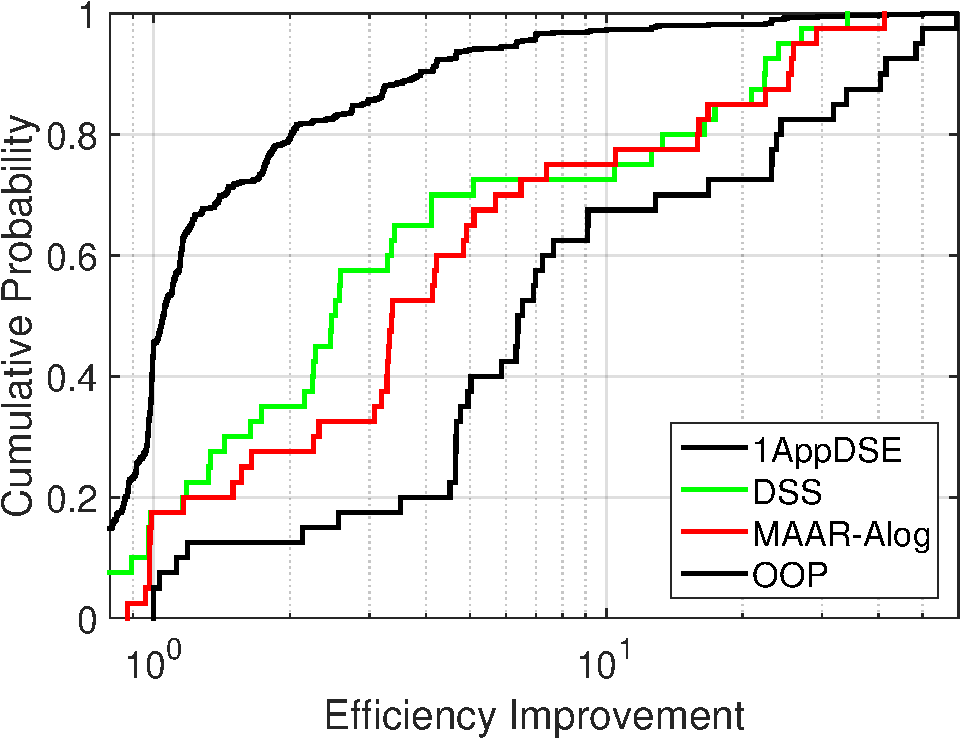
\includegraphics[width=.48\linewidth]{fig/MAARsw12all.pdf}\label{fig:sw12all}}
		\hfill
		\subfloat[Efficiency Achievement] {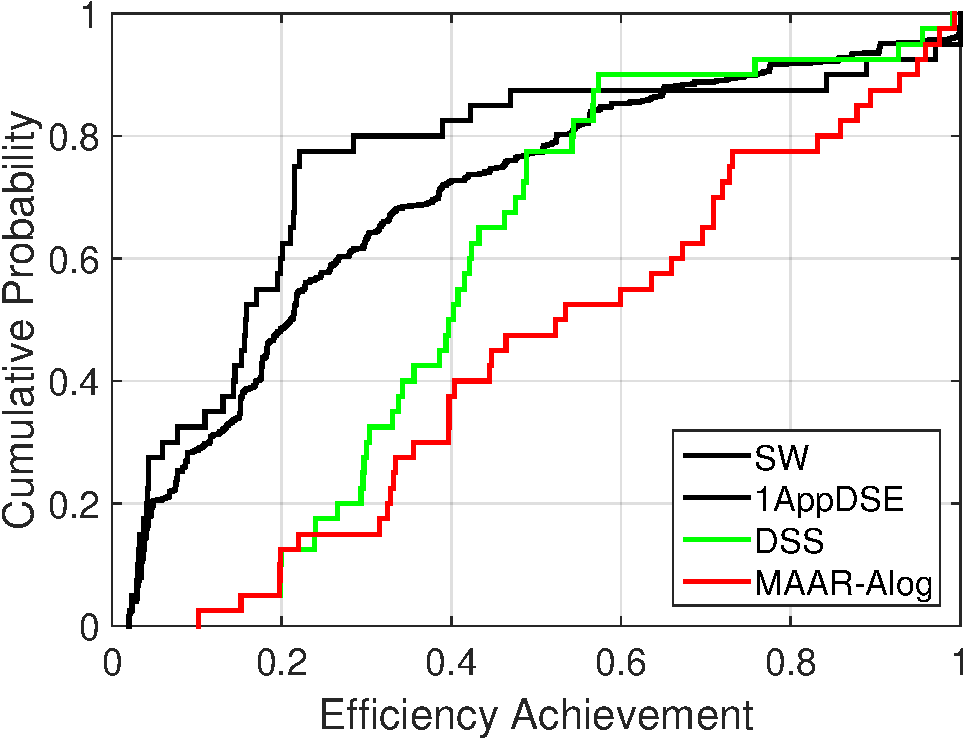
\includegraphics[width=.48\linewidth]{fig/MAARoop12all.pdf}\label{fig:oop12all}}
		\vspace{-8pt}
	\caption{Cumulative Probability with 12 ACCs Budget}
	\label{fig:all12}
		\vspace{-0pt}
\end{figure}

To give a broader comparison with 1AppDSE and DSS, 
\figref{fig:all12} highlights MAAR's benefits for a ACCs=12 budget. Note that 1AppDSE shows more detail as it considers runing any app on any app's dedicated OPT platform. In \figref{fig:sw12all}, MAAR improves efficiency more than 1appDSE and DSS for almost all applications. 
67.5\% of applications have at least a 3x improvements, while 1appDSE and DSS only improve 15\% and 42.5\% of applications respectively by the same amount. In \figref{fig:oop12all}, MAAR has a significantly higher achievement than 1appDSE and DSS. 55\% of applications obtain at least 60\% of their dedicated OPT platform (1appDSE: 20\%, DSS 15\%).

\tabref{tab:maar} shows MAAR DSE benefits when designing one platform for the OpenVX market with 1 to 6 ACCs. 
%gives insight on which OpenVX kernels MAAR chooses for a platform with 1 to 6 ACCs, as well as how often each ACC is used. 
All kernels are compute intense yielding a high efficiency improvement if accelerated. \textit{Custom Convolution} is most frequently used (39 times) as it is the basis of many vision kernels. For a platform with 2 ACCs, MAAR adds \textit{Canny Edge} (9 times used). Overall, kernels appearing more frequently are not necessarily selected by MAAR DSE. Sometimes, less frequent but compute-intensive functions, e.g. \textit{Optical Flow Pyramid (LK)} added as a 4th ACC, have a higher priority.
However, this also indicates some limits of the input DFGs which were derived from the app's OpenVX calls. This kernel could be decomposed in many smaller kernels, which then subsequently could be reused more. 
%
Considering the specialization of kernels, e.g. \textit{Gaussian Filter} is a specialization of \textit{Convolution} which takes advantage of weight symmetries, is part of the future work.


\vspace{-2pt}

\begin{table}[h]
	\caption{MAAR Kernel Allocation}
	\label{tab:maar}
	\vspace{-8pt}
	\centering
	\begin{tabular}{|P{0.15\linewidth} | P{0.5\linewidth} | P{0.15\linewidth}|}
		\toprule
		\#ACCs & ACC Kernel Added & \#Used \\
		\midrule
		\hline
		1 & Custom Convolution & 37 \\
		\hline
		2 & Canny Edge Detector & 9 \\
		\hline
		3 & Harris Corners & 7 \\
		\hline
        4 & Optical Flow Pyramid (LK) & 4 \\
        \hline
        5 & Box Filter & 7 \\
        \hline
        6 & Gaussian Filter & 9\\
		\bottomrule
	\end{tabular}
\end{table}

\vspace{-2pt}

% the order of kernel in OpenVX allocation. CustomConvolution CannyEdgeDetector HarrisCorners OpticalFlowPyramid(LK)  BoxFilter GaussianFilter


MAAR DSE design run-time is very moderate thanks to the fast heuristic GA traversal and a fast evaluation. Exploring a common platform with ACCs=19 for the 40 OpenVX applications on a 3.10GHz Intel i5-3450 only takes 147.56s.



